With the view to implement both Zero Trust smart home architectures, which were previously introduced, this chapter describes their step by step implementation, while also aiming to answer the practical research questions on whether the Zero Trust paradigm is suitable to be integrated into smart homes, and whether a smart home network should be hosted locally or in the cloud.\\
Both implementations offer a similar security configuration, utilizing multi-factor authentication through the Cisco Duo MFA provider, which offers a simplistic and user-friendly solution \cite{duo_mfa}. Additionally, the introduction of filtering of the incoming traffic -- locally based on the user IP address over the remote VPN tunnel, as part of the Cloudflare Zero Trust service \cite{cloudflare_zt} and in the cloud through exclusively allowing traffic over specific ports, as well as the integration of an IP ban further serve as security measures.

\section{On-Premise Architecture Implementation}
Beginning with the on-premises implementation, its smart home architecture has been designed to be a purely local one, integrated it into the university network of the FH Aachen and exclusively within its IP address range. Hardware wise, it has been implemented using a Raspberry Pi SBC as a host device, together with the necessary accessories, as depicted in Figure 4.1.
\begin{figure}[H]
	\centering
	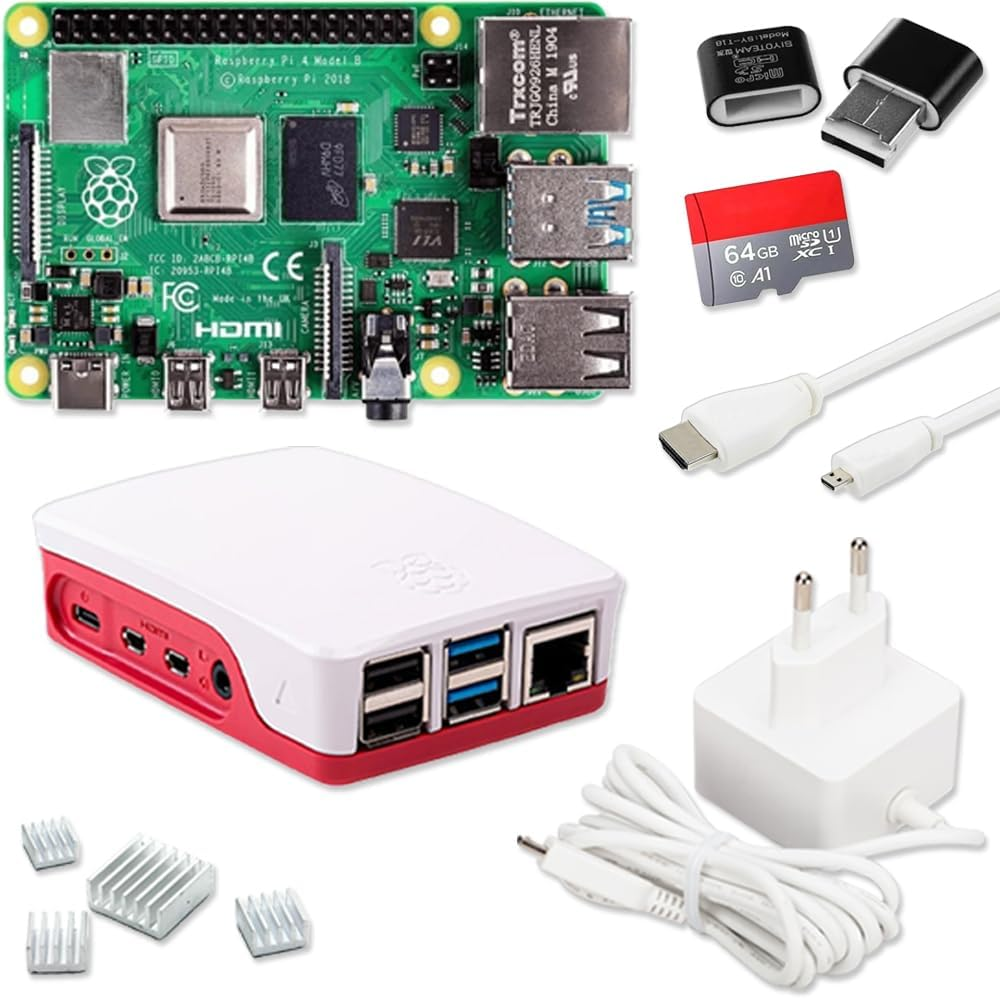
\includegraphics[width=0.4 \linewidth]{Images/K4/hardware-rpi.jpg}
	\caption{Main Components of a Raspberry Pi Starter Set}
	\label{fig:Rpi_set}
    \cite{rpi_starter}
\end{figure}

\subsubsection{Installation}
Firstly, the first step of the project was utilizing the Raspberry Pi Imager \cite{rpi_imager_gh} (Figure 4.2.) to load an image of the Home Assistant OS (HAOS) onto an SD card and inserting it into the Raspberry Pi. After RPI Imager had finished loading the OS, the RPI itself was booted with the modified SD card. After a short duration of ca. 10 minutes, the RPI was fully operational running HAOS and hosting the Home Assistant starting page to begin the onboarding, as depicted in Figure 4.3. The HA instance was accessible under the \textit{homeassistant.local:8123} URL under the 8123 default port. 
\begin{figure}[H]
	\centering
	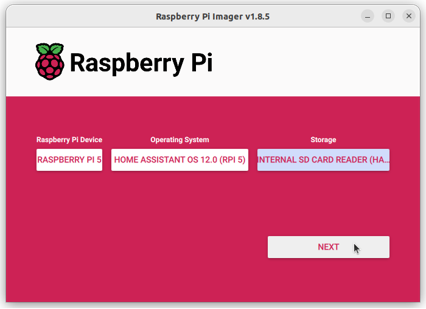
\includegraphics[width=0.6 \linewidth]{Images/K4/Picture1.png}
	\caption{Raspberry Pi Imager}
	\label{fig:Rpi_ha}
    \cite{rpi_imager_ha}
\end{figure}

\begin{figure}[H]
	\centering
	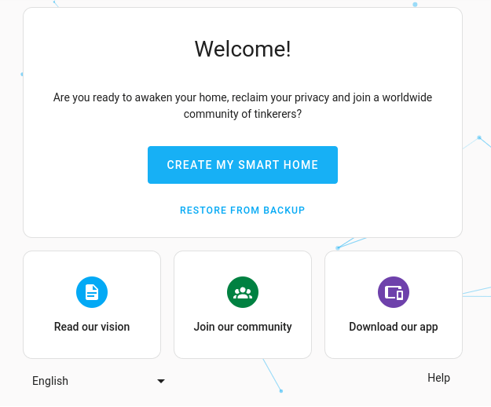
\includegraphics[width=0.6 \linewidth]{Images/K4/Picture2.png}
	\caption{Home Assistant Start Page}
	\label{fig:Rpi_start_ha}
    \cite{rpi_ha_onboarding}
\end{figure}

After the installation is complete, the user is walked through the creation of their first profile by being required to enter their username and password, as depicted in Figure 4.4. It should also be noted that while the onboarding process is very straightforward and easy to follow, it can lack security-conscious messages for passwords. Beyond a simple text under the text field, there is no indication that the user is creating a secure password, as defined in \cite{bsi_secure_pass}.
After a short loading time, the user is greeted by the default Home Assistant dashboard (Figure 4.5.).

\begin{figure}[H]
	\centering
	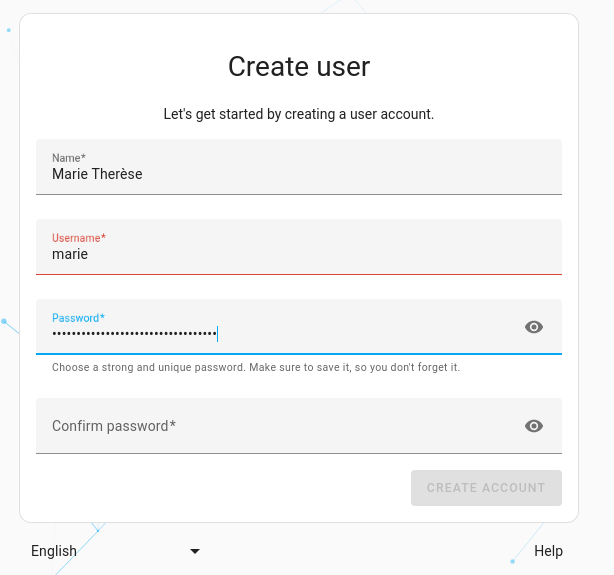
\includegraphics[width=0.5 \linewidth]{Images/K4/Picture4.png}
	\caption{User Profile Creation in Home Assistant}
	\label{fig:Rpi_user}
    \cite{rpi_ha_onboarding}
\end{figure}

\begin{figure}[H]
	\centering
	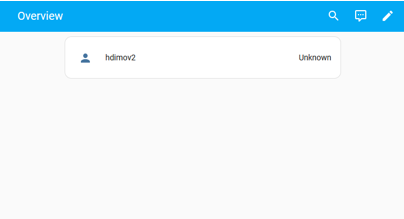
\includegraphics[width=0.5 \linewidth]{Images/K4/Picture5.png}
	\caption{Home Assistant Default Dashboard}
	\label{fig:Rpi_dashboard}
\end{figure}

By delving into the settings, it is apparent that upon the installation completion, there has automatically been a full backup of the system created (Figure 4.6.), establishing an initially straightforward and automatic backup process.

\begin{figure}[H]
	\centering
	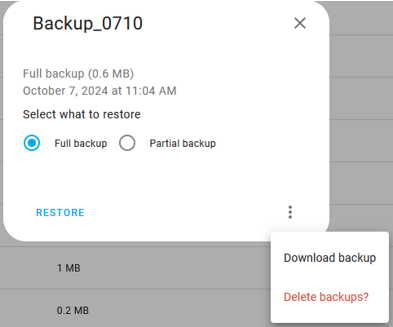
\includegraphics[width=0.4 \linewidth]{Images/K4/Picture3.png}
	\caption{Backup Instance Details}
	\label{fig:Rpi_backup}
\end{figure}


\subsection{Configuration}
With the view to introduce the configuration of the security features for this environment in more detail, the first one to be configured was the MFA process for the user login. After integrating the MFA provider Cisco Duo for the distribution of a TOTP for each login with a 30-second time limit from the client device, the login process can be described in three simple steps:
\begin{enumerate}
    \item \textit{Enter username and password.}
    \item \textit{Enter TOTP from client device.}
    \item \textit{Access login page.}
\end{enumerate}

As the configuration under Home Assistant is concentrated in a single \textit{configuration.yaml} file \cite{rpi_ha_config}, the integration of an MFA process is carried out in a centralized manner. To describe the process, firstly, the user enters the following lines in the config file, as shown in Figure 4.7. It is noteworthy that the configuration code may differ, depending on the type of second factor added and MFA provider \cite{ha_mfa}.
\begin{figure}[H]
	\centering
	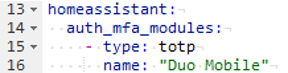
\includegraphics[width=0.4 \linewidth]{Images/K4/Picture8.png}
	\caption{Home Assistant MFA YAML Configuration}
	\label{fig:Rpi_config}
\end{figure}

Subsequently, the user links the MFA provider application (e.g. Duo Mobile) on the client device by scanning a temporary quick-response (QR) code, provided in the Home Assistant settings for the introduction of a second authentication factor, as depicted in Figure 4.8.
\begin{figure}[H]
	\centering
	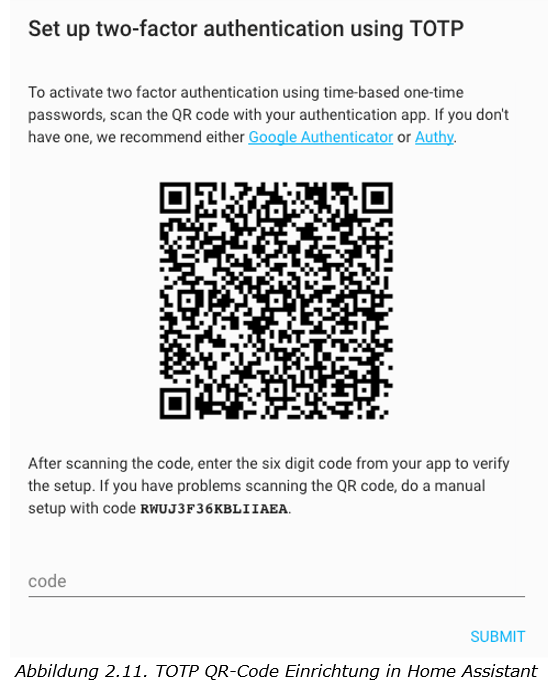
\includegraphics[width=0.5 \linewidth]{Images/K4/Picture8-1.png}
	\caption{Home Assistant MFA QR Code Example}
	\label{fig:Rpi_qr}
\end{figure}

The next feature to be implemented is an IP ban on all IP addresses, which have failed to authenticate themselves properly, exceeding a certain login attempt threshold. This feature is implemented the same way, by entering the lines, depicted in the Figure 4.9.
\begin{figure}[H]
	\centering
	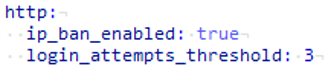
\includegraphics[width=0.5 \linewidth]{Images/K4/Picture12.png}
	\caption{Home Assistant IP Ban Configuration}
	\label{fig:Rpi_ban}
\end{figure}

After a successful IP address ban a so-called block list file, \textit{ip\_bans.yaml}, has been created in the configuration folder containing the banned client IP address with a timestamp (Figure 4.10.), being updated over time with banned IP addresses. After being banned, the user receives a 403 status code, forbidding them from visiting the page, as depicted in Figure 4.11.
\begin{figure}[H]
	\centering
	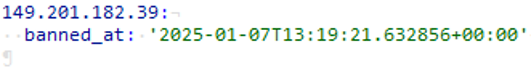
\includegraphics[width=0.6 \linewidth]{Images/K4/Picture13.png}
	\caption{Home Assistant IP Ban Blocklist}
	\label{fig:ha_blocklist}
\end{figure}
\begin{figure}[H]
	\centering
	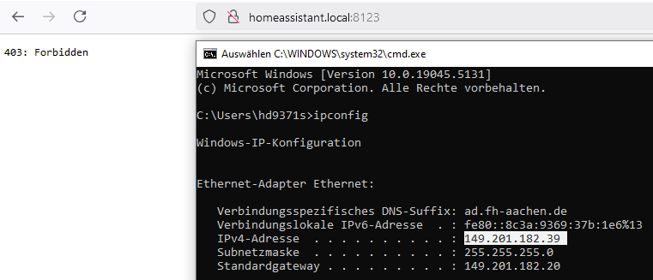
\includegraphics[width=0.7 \linewidth]{Images/K4/Picture14.png}
	\caption{Home Assistant User Ban}
	\label{fig:ha_ban}
\end{figure}

Another feature implemented in the on-premise environment is the remote tunnel over a VPN connection, connecting the Home Assistant instance with the Internet. Figure 4.12. depicts the added lines to the \textit{configuration.yaml} file as the first step to implement the tunnel. The configuration file should include the list of trusted proxy IP addresses, allowed to access the remote tunnel \cite{ha_proxies}. 

\begin{figure}[H]
	\centering
	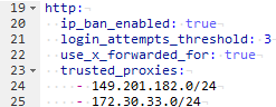
\includegraphics[width=0.5 \linewidth]{Images/K4/Picture15.png}
	\caption{Home Assistant Remote Tunnel YAML Configuration}
	\label{fig:tunnel_config}
\end{figure}

By creating the remotely managed tunnel connection using Cloudflare Zero Trust \cite{cloudflare_zt_tunnel}, the user receives a Cloudflare tunnel token. Together with the name of the tunnel, they are saved in the Cloudflare tunnel client, utilized by Home Assistant as an add-on \cite{ha_cloudflared}. Figure 4.13. represents the details about the tunnel from the Cloudflare dashboard, while figure 4.14. shows the add-on configuration window with the tunnel URL, Cloudflared tunnel name and token.
\begin{figure}[H]
	\centering
	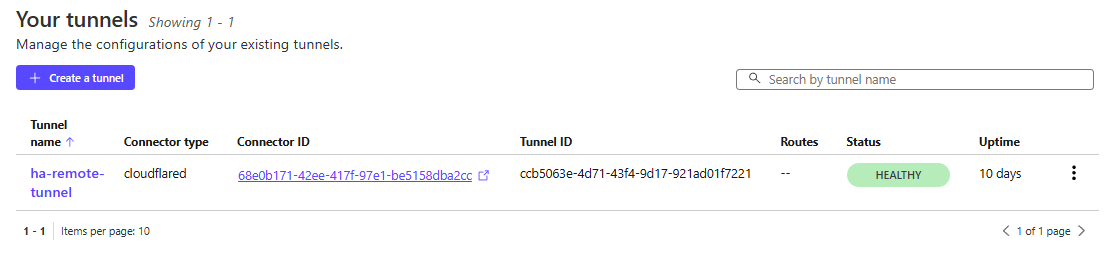
\includegraphics[width=1 \linewidth]{Images/K4/ha-tunnel-k4.png}
	\caption{Remote Tunnel Dashboard}
	\label{fig:tunnel_dash}
\end{figure}
\begin{figure}[H]
	\centering
	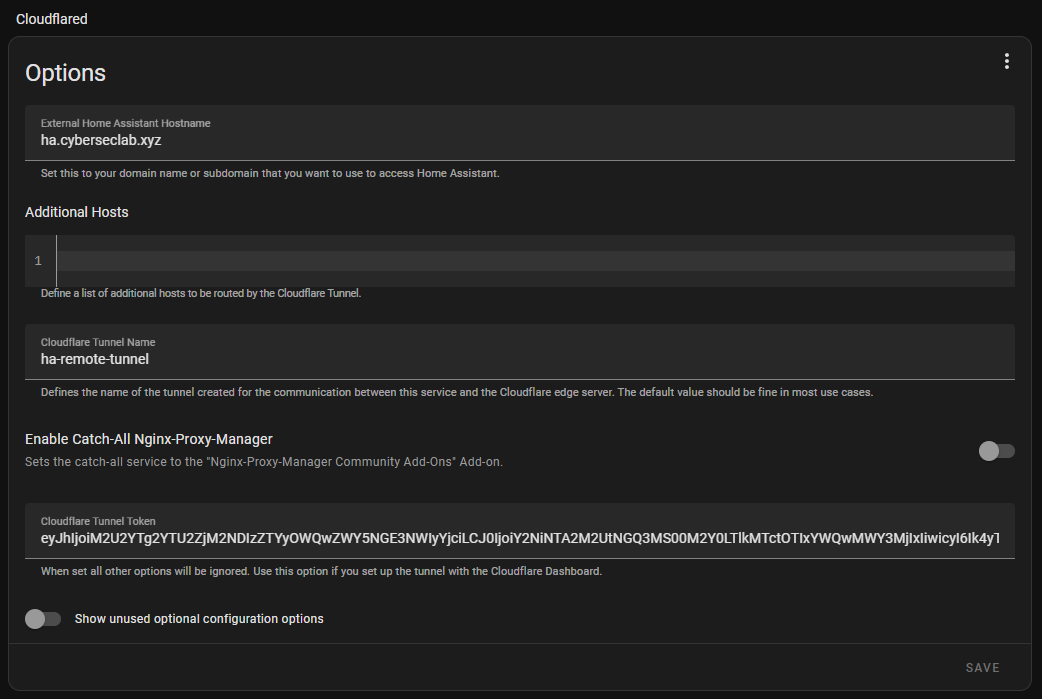
\includegraphics[width=0.8 \linewidth]{Images/K4/cloudflared-config.png}
	\caption{Cloudflared Tunnel Configuration}
	\label{fig:ha_cloudflared}
\end{figure}

After the tunnel has been configured, the following two firewall rules have been implemented with special syntax over the Cloudflare UI:
\begin{itemize}
    \item \textit{(ip.geoip.country ne "DE")}: All IP Addresses not registered in Germany are blocked from accessing the tunnel.
    \item \textit{(not ip.src in uni\_network)}: All IP Addresses not part of the university network are blocked from accessing the tunnel.
\end{itemize}

Figure 4.15. depicts an example of a user not being able to access the tunnel, since they fulfil either of the criteria of the aforementioned blocklists.
\begin{figure}[H]
	\centering
	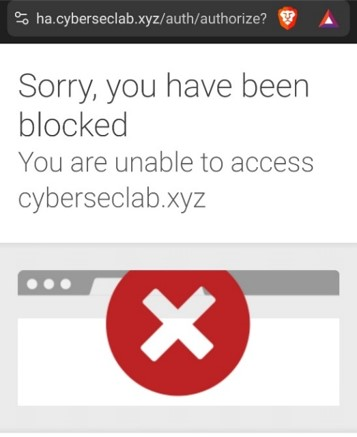
\includegraphics[width=0.4 \linewidth]{Images/K4/Picture19.jpg}
	\caption{Remote Tunnel Access Error}
	\label{fig:tunnel_error}
\end{figure}

\subsection{Structure \& Device Integration}
In its entirety, the on-premise architecture is depicted in Figure 4.16., which provides a high-level view of the user and design workflow within the environment. The user has access to the local smart home environment directly either by an SSH tunnel connection or using the default local connection, or the remote tunnel connection by way of a VPN. Inside the local area network, the Home Assistant instance utilizes a Zigbee gateway connection to connect to the set of IoT devices, paired within the network.
\begin{figure}[H]
	\centering
	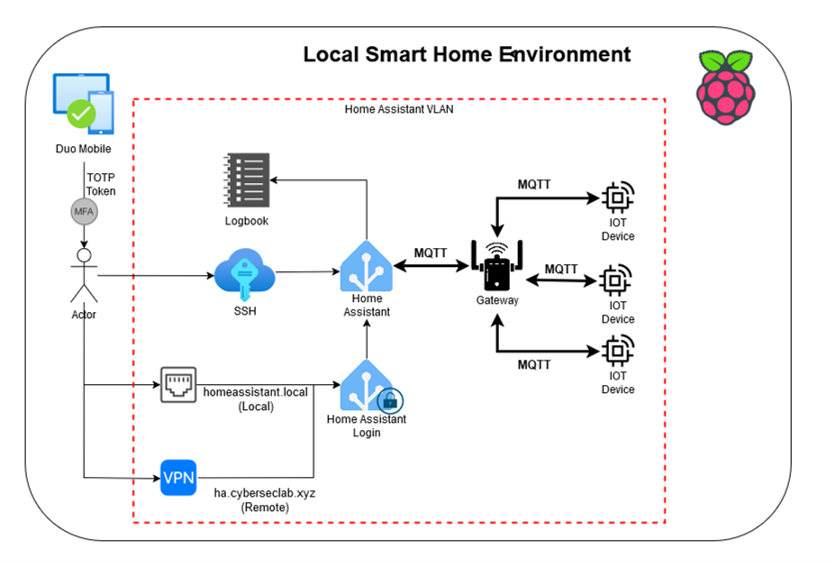
\includegraphics[width=0.8 \linewidth]{Images/K4/Picture21.png}
	\caption{Architecture Diagram of On-Premise Environment}
	\label{fig:local_arch}
\end{figure}

The integration of the following IoT devices has been carried out over the Zigbee and BLE protocols:
\begin{itemize}
    \item 1 TVOC air quality sensor\cite{aqara_monitor}
    \item 2 IKEA Tradfri LED bulbs\cite{tradfri_led}
    \item 1 IKEA Tradfri power outlet\cite{tradfri_outlet}
    \item 1 Flower care plant sensor\cite{flower_care_sensor}
\end{itemize}

All IoT devices except the Flower care plant sensor communicate over the Zigbee with the gateway, while the flower sensor uses the integrated BLE protocol.\\
With regards to the functionality of the devices, the IKEA Tradfri devices are switched on and off from the Home Assistant dashboard. In addition, 2 automations have been created with this setup. One of the Tradfri light bulbs flashes shortly after the Tradfri socket is switched on, while the other automation has been implemented as a troubleshooting mechanism, flashing when the Zigbee gateway is connected to Home Assistant. Figure 4.17. depicts the aforementioned devices within the local environment dashboard.
\begin{figure}[H]
	\centering
	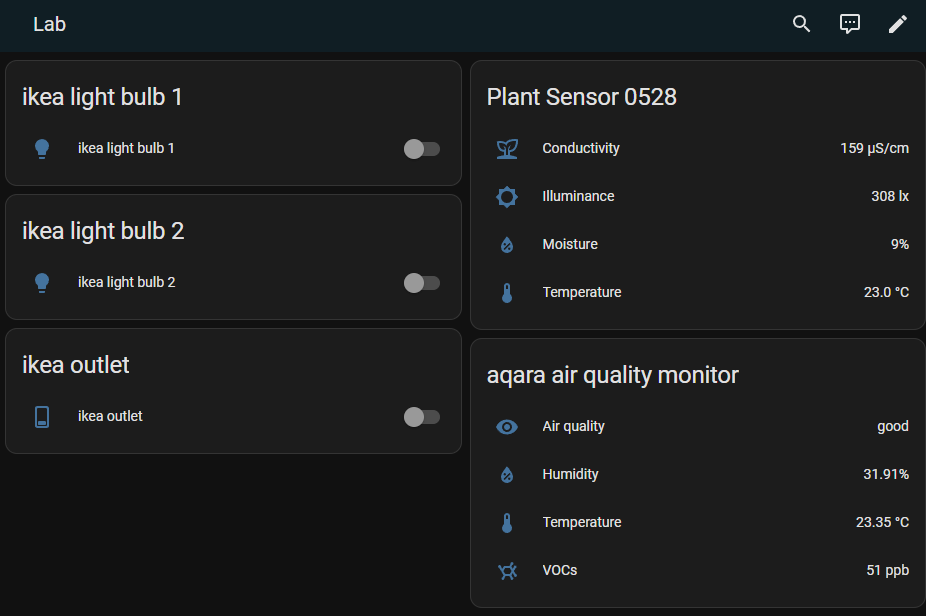
\includegraphics[width=0.7 \linewidth]{Images/K4/ha-dashboard-2.png}
	\caption{Home Assistant Devices Dashboard}
	\label{fig:ha_dashboard}
\end{figure}

\section{Cloud-based Architecture Implementation}
Regarding the cloud-based architecture, it has been implemented by utilizing the AWS Elastic Compute Cloud service as a VM, together with Terraform to provision the needed infrastructure and Docker Compose to start the Home Assistant application in a container. Figure 4.18. depicts the concept diagram for the environment's structure.
The user has two ways of accessing the HA software instance, either by the MFA login process or over an SSH session.\\
What separates this environment from the local one in terms of functionality, is the lack of integrated IoT in the environment, since the process of pairing a device with the host device is more complicated for the cloud-based SHS. The "Outlook" section of Chapter 6 addresses how this process could be realized by using AWS IoT services.

\begin{figure}[H]
	\centering
	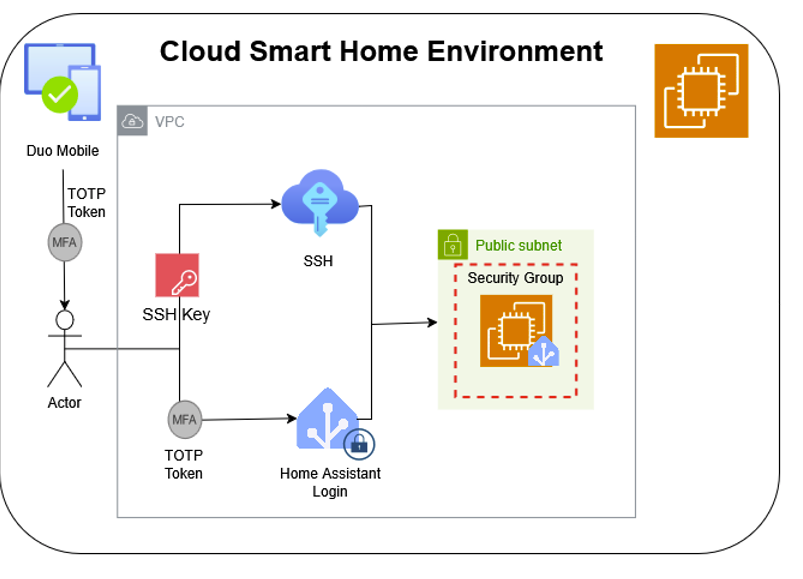
\includegraphics[width=0.8 \linewidth]{Images/K4/Picture42.png}
	\caption{Architecture diagram of cloud-based environment}
	\label{fig:cloud_arch}
\end{figure}

\subsection{Configuration}
To review the configuration process, as already mentioned, the configuring the cloud environment is mostly managed over Terraform as an IaC tool. This is achieved by writing configuration files for the instance's provisioned infrastructure -- defining the desired state of the system. A simple example is depicted in the \textit{main.tf} file (Figure 4.19) as part of the cloud setup, depicting the definition of the EC2 instance under the \textit{"aws\_instance" "ec2\_vm"} resource and an output of its public IP address every time changes to the terraform scripts are applied \cite{tf_output}, as Figure 4.20 depicts.
\begin{figure}[H]
	\centering
	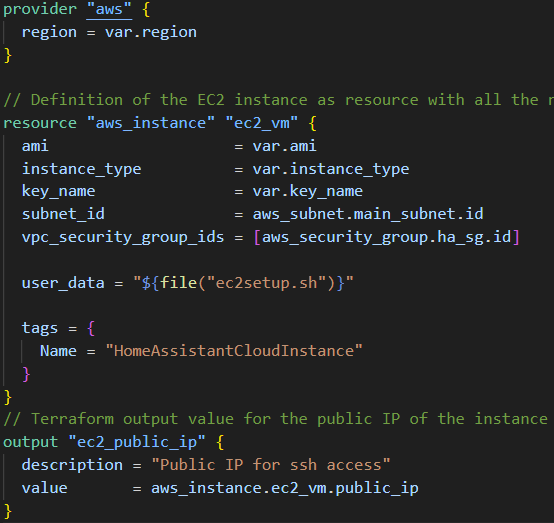
\includegraphics[width=0.7 \linewidth]{Images/K4/Picture29.png}
	\caption{main.tf of cloud environment configuration}
	\label{fig:main_tf}
\end{figure}
\begin{figure}[H]
	\centering
	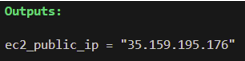
\includegraphics[width=0.4 \linewidth]{Images/K4/Picture30.png}
	\caption{Terminal output after applying script changes}
	\label{fig:main_tf_output}
\end{figure}

All the specific information about the EC2 instance and its configuration is accessible from the variables, defined in two separate variable files. The first file, \textit{variables.tf} (Figure 4.21.) declares the variables and provides individual descriptions. On the other hand, the \textit{terraform.tfvars} file (Figure 4.22.) is where all variable values are set, making it the more crucial file of the two. It specifically defines the network as part of the Virtual Private Cloud (VPC) of an EC2 instance and the VPC default components \cite{tf_vpc_components}, containing the essential data, e.g. the subnet and CIDR distribution, availability zones, AMI image ID and the instance type.
\begin{figure}[H]
	\centering
	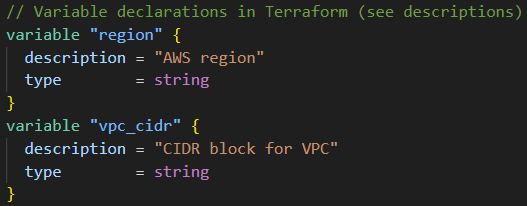
\includegraphics[width=0.7 \linewidth]{Images/K4/Picture32.png}
	\caption{variables.tf}
	\label{fig:var_tf}
\end{figure}
\begin{figure}[H]
	\centering
	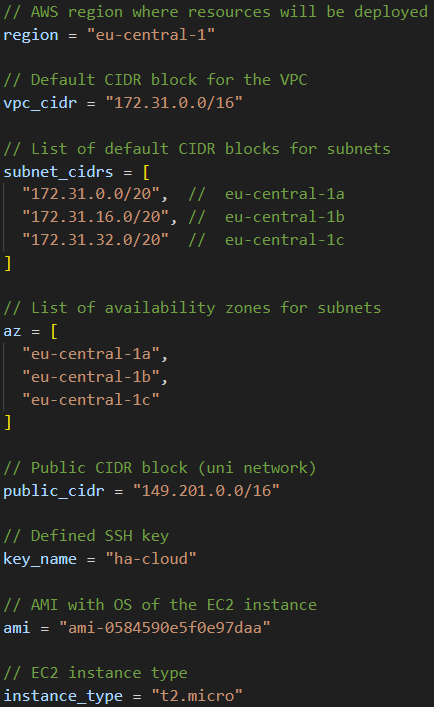
\includegraphics[width=0.5 \linewidth]{Images/K4/Picture33.png}
	\caption{terraform.tfvars}
	\label{fig:tf_vars}
\end{figure}

As regards the security settings, they are most commonly allocated in terraform through resources, in the same way as the EC2 instance. For instance, to configure the incoming and outgoing traffic for the EC2 instance the user defines the \textit{aws\_security\_group} resource, as depicted in Figure 4.23. 
In this instance, the security group is connected to the CIDR block of the current VPC to allow the incoming traffic over the ports 22 (SSH) and 8123 (Home Assistant) from a specific public CIDR group of IP addresses through the definition of these rules as additional resources, while allowing outgoing traffic to the constraints of the local network. These settings are also visible from the AWS EC2 instance dashboard, as Figure 4.24. depicts.
\begin{figure}[H]
	\centering
	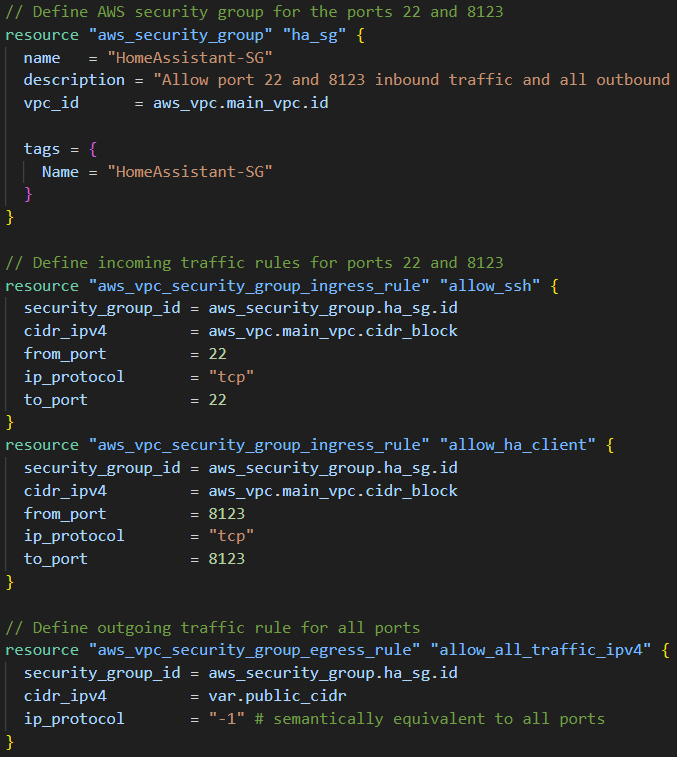
\includegraphics[width=0.8 \linewidth]{Images/K4/Picture36.png}
	\caption{HomeAssistant-SG Security Group}
	\label{fig:tf_sg}
\end{figure}

\begin{figure}[H]
	\centering
	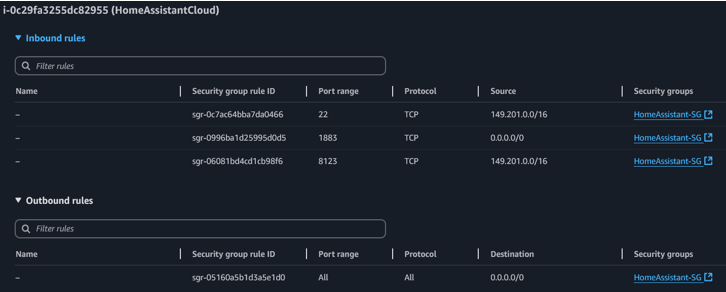
\includegraphics[width=1 \linewidth]{Images/K4/Picture35.png}
	\caption{HomeAssistant-SG in the AWS Dashboard}
	\label{fig:tf_sg_aws}
\end{figure}

With the aim to set up the smart home environment, a starter script can be passed over the \textit{user\_data} attribute in Terraform, as if the user itself has entered commands in the CLI. The purpose of this script is to automatically install the default packages needed for the VM to run Home Assistant in a Docker Compose container setup \cite{compose_install}, as well as provide the starter configuration for the \textit{docker-compose.yml} file, on which Docker Compose bases the HA application deployment. The container is then started at the end of the script, allowing the user to access the Home Assistant instance over its public IP address and the 8123 port through the FH Aachen network. According to Figure 4.20. this is \textit{35.159.195.176:8123}, however the IP address may vary. Figure 4.25. depicts the starter configuration script for the EC2 instance in AWS.

\begin{center}
  \label{fig:ec2setup}
\end{center}
\inputminted[breaklines, linenos]{bash}{Code/tf_config/ec2setup.sh}
\captionof{figure}{EC2 Instance Setup Script}

\section{Conclusions}
To complete the chapter outlining the implementation of both security smart home architectures, there are several key conclusions that have been drawn from their practical realization as ZT starting configurations. This section provides a brief overview of each of those aspects, which are then further expanded upon in the evaluation of this work in the overall assessment of this work according to the evaluation metrics defined in Chapter 3.

\subsubsection{Environment Setup}
When assessing either the on-premise or the cloud-hosted environment, it should be kept in mind that while they offer a starting configuration for a Zero Trust architecture in smart homes, their setup process is different.\\

With regard to the local environment, the duration of the start-up phase (defined in Chapter 3) can be longer, as the user will need to obtain their own host device (e.g. Raspberry Pi), as well as install the HA software, which will manage the IoT devices within the environment. Moreover, one of the central components of the on-premise environment are the Home Assistant add-on applications \cite{ha_addons}, which even though they are easy to install and contribute to the integration of security measures, may cause a fundamental security risk. This is because the vast majority of them are open-source and cannot be subject to security guarantees.\\

In contrast to that, the cloud environment is relatively swift to set up. The combination of AWS and Terraform as an IaC tool offers a way for users to organize every aspect of the environment in a straightforward way. The provisioned VM negates the need to acquire a separate host device and utilizing a one-time setup script together with Terraform, with its approach to define the desired end state of the configuration, is a way to minimize the time it takes to have a starter smart home environment.

\subsubsection{Device Integration}
As regards the topic of device integrations for both environments, they also differ in their complexity.
Integrating devices locally is a straightforward process of the device being in proximity to the host device. This offers an advantage when it comes to the ease of use of the SHS.\\

When it comes to the cloud-hosted environment, the process of pairing an IoT device is by all means a more complex one and has not been practically realized. Since the central part of the SHS is a host device, which is remotely provisioned by an IaaS provider, it is not plausible to integrate a device by the traditional means of closeness. The concept of a virtual gateway hosted by the host device (in this case a Raspberry Pi) offers a potential solution to that problem, however from a security perspective, it should be further investigated. As it stands, the current configuration of the cloud environment cannot integrate an IoT device, the implications of which are further explored in the next chapter. 